\documentclass[border=2mm]{standalone}
\usepackage{pgfplots}
\usepackage[scaled]{helvet}
\usepackage[T1]{fontenc}
\renewcommand\familydefault{\sfdefault}
\usepackage[eulergreek]{sansmath}
\pgfplotsset{
tick label style = {font=\sansmath\sffamily}}

\pgfkeys{/pgf/number format/fixed}
\pgfplotsset{compat=newest}

\begin{document}

\pgfplotsset{
colormap={whitered}{color(0cm)=(white); color(1cm)=(orange!75!red)}}

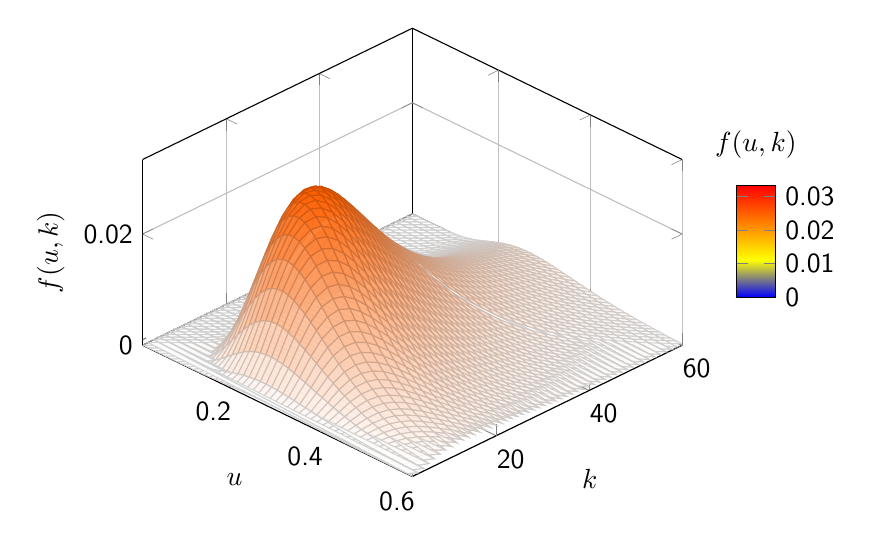
\begin{tikzpicture}[
    declare function={mu1=-1.2;},
    declare function={mu2=3.1;},
    declare function={sigma1=sqrt(0.25);},
    declare function={sigma2=sqrt(0.9);},
    declare function={bivar(\ma,\sa,\mb,\sb)=1/(2*pi*x*y*\sa*\sb) * exp(-((ln(x)-\ma)^2/\sa^2+(ln(y)-\mb)^2/\sb^2))/2;}]
\begin{axis}[
    view={45}{45},
    enlargelimits=false,
    grid=major,
    domain=0:0.6,
    y domain=2:60,
    samples=200,
    xlabel=$u$,
    ylabel=$k$,
    zlabel={$f(u,k)$},
    scaled z ticks=false,
    colorbar,
    colorbar style={
        at={(1.1,0.4)},
        anchor=south west,
        height=0.25*\pgfkeysvalueof{/pgfplots/parent axis height}, scaled ticks=false,
        title={$f(u,k)$}
    }
]
\addplot3 [surf, opacity=0.8,fill opacity=0.9,colormap={whitered}{color(0cm)=(white); color(1cm)=(orange!75!red)}, samples=50] {bivar(mu1,sigma1,mu2,sigma2)};

\draw [black!50] (axis cs:-1,0,0) -- (axis cs:4,0,0);
\draw [black!50] (axis cs:0,-1,0) -- (axis cs:0,4,0);

\end{axis}
\end{tikzpicture}
\end{document}